\documentclass[11pt]{article}
% ---------------------------------------------------------------- packages
\usepackage[letterpaper, margin=1in]{geometry}
\usepackage[T1]{fontenc}
\usepackage{newtxtext, newtxmath}
\usepackage{microtype}
\usepackage{amsmath}
\usepackage{graphicx}
\usepackage{booktabs}
\usepackage{xcolor}
\usepackage[font=small, labelfont=bf, skip=4pt]{caption}
\usepackage[numbers, sort&compress]{natbib}
\usepackage{enumitem}
\usepackage{fancyhdr}
\usepackage{float}
\usepackage[section]{placeins}
\usepackage[colorlinks=true, linkcolor=blue!50!black, citecolor=blue!50!black, urlcolor=blue!50!black]{hyperref}
\graphicspath{{figures/}}
\setlist{itemsep=1pt, topsep=3pt}
\setlength{\emergencystretch}{2em}
\renewcommand{\topfraction}{0.9}
\renewcommand{\bottomfraction}{0.8}
\renewcommand{\textfraction}{0.07}
\renewcommand{\floatpagefraction}{0.8}
\definecolor{boxbg}{HTML}{F3F6FA}
\setlength{\textfloatsep}{12pt plus 2pt minus 2pt}
\pagestyle{fancy}
\fancyhf{}
\renewcommand{\headrulewidth}{0pt}
\fancyfoot[C]{\thepage}
\newcommand{\tabin}[1]{\csname @@input\endcsname tables/#1 }

\title{\textbf{Reading Backdoors from Weights:\\Can Language-Model Agents Detect and Remove\\Neural Trojans by Inspecting and Editing Parameters?}}
\author{Yukteswar}
\date{November 11, 2026}

\begin{document}
\maketitle
\thispagestyle{fancy}

\begin{abstract}
A backdoored neural network behaves normally on ordinary inputs but obeys a hidden trigger. We ask
whether a large language model (LLM) can audit such a network the way a human expert might: by
\emph{reading} its weights to decide whether it is backdoored, and by \emph{editing} its weights to
remove the backdoor. To answer this with known ground truth, we train a zoo of 120 small CIFAR-10
convolutional networks (24{,}234 parameters each), half of them poisoned with BadNets-style patch
triggers, and compare openly available LLMs (NVIDIA Nemotron~3 Ultra and Nemotron~3.5 Super VL)
against seven conventional defences under matched access. Reading is hard for the LLM: from the
weights alone, as text or as images, it separates backdoored from clean networks only slightly
better than chance (AUROC 0.61--0.65, against 0.87--0.94 for weight statistics and Neural Cleanse),
because it calls most networks backdoored. Writing goes much better. Given a Python sandbox with the
weights, 1{,}000 clean images and a budget of 50 forward passes but no gradients, the LLM agent
probes the network with patches it designs itself, locates the neuron that carries the trigger, and
edits a median of six weights. It removes the backdoor outright (attack success below 20\%) in 6 of
20 networks, more than any baseline, with a mean attack success of 51.9\% against 42.8\% for the best
baseline. Ablations, each repeated three times, show where this comes from: an agent that can only
probe the network does worse (60.4\% averaged over runs, against 50.4\% for the full agent, $p=0.009$),
one that can only read the weights does much worse (77.1\%) yet reproduces the full agent's edit on
the clearest case, and the same edits moved to random positions do nothing (89.5\%). Single runs vary
widely: the agent removes 11 different backdoors across three runs, but only one in every run. The agent and the best baseline fail on different networks,
which points to LLM-guided repair as a complement to, not a replacement for, classical defences. All code, models, transcripts and figures are released.
\end{abstract}

% ============================================================================
\section{Introduction}
Pretrained networks are routinely downloaded, fine-tuned and redistributed. This supply chain is
open to \emph{backdoor} (trojan) attacks~\citep{gu2017badnets}: an attacker poisons a small fraction
of the training data with a trigger pattern relabelled to a target class. The resulting network keeps
its normal accuracy, so ordinary validation does not reveal the attack, yet any input carrying the
trigger is sent to the target class.

Most defences treat the network as a black box to be probed with data: they reverse-engineer a
candidate trigger for every class~\citep{wang2019neuralcleanse}, prune neurons that stay quiet on
clean data~\citep{liu2018fineprune}, or inspect activations~\citep{tran2018spectral}. A second line
of work treats \emph{weights as data} and trains predictors that take a network's parameters as
input~\citep{unterthiner2020predicting, schurholt2022modelzoos, navon2023equivariant, xu2021mntd}.
Neither line uses the kind of open-ended, hypothesis-driven inspection that a human expert would
apply to a suspicious model: look at the weights, notice something odd, design an experiment,
and fix exactly the part that is broken.

Large language models now read long technical inputs, write and run code, and act in loops of
reasoning and tool use~\citep{yao2023react, schick2023toolformer}. They have also been used to
describe what individual neurons do~\citep{bills2023explain}. This raises a direct question:
\emph{can an LLM audit a network by reading its weights, and repair it by editing those weights?}

\paragraph{How the project developed.} The study was built in three stages
(Figure~\ref{fig:overview}). First, we built a controlled testbed: a zoo of small CNNs, half of
them poisoned by us, so that every question has a known answer. Second, we measured strong
non-LLM baselines on it, which fixed the bar any LLM result must clear. The LLM protocol was written
at the same time, before any LLM was run. Third, we ran the LLM experiments. The protocol was
first specified for a frontier commercial model; to keep the study free to reproduce, it was run
on openly available Nemotron models through NVIDIA's free API catalog~\citep{nvidia2026catalog},
starting with a two-model pilot to check the input length, the tool loop and the rate limits.

\begin{figure}[!htb]
  \centering
  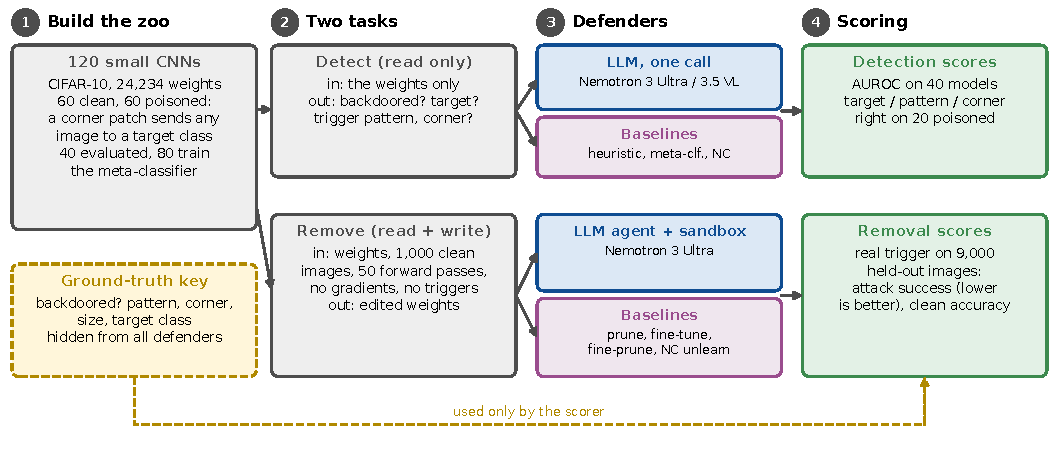
\includegraphics[width=\linewidth]{overview.pdf}
  \caption{\textbf{Study design.} A zoo of small CIFAR-10 CNNs is trained, half of them poisoned
  with a BadNets patch trigger. Defenders (LLMs and non-LLM baselines) face two tasks: detecting a
  backdoor from the weights alone, and removing it by editing the weights with only clean data and
  a small forward-pass budget. The ground-truth key is written at training time and used only by the
  scorer.}
  \label{fig:overview}
\end{figure}

\paragraph{Contributions.}
\begin{enumerate}[leftmargin=*]
  \item \textbf{A weight-space auditing testbed} (Section~\ref{sec:testbed}): 120 CIFAR-10 networks
    small enough that every weight fits in one LLM prompt, with training settings sampled
    identically for clean and poisoned models and ground truth kept apart from anything a defender
    sees.
  \item \textbf{Two protocols for LLMs to work on raw weights} (Section~\ref{sec:llm}):
    \emph{reading}, where the LLM sees all weights as text or images and answers in one call, and
    \emph{writing}, where an LLM agent edits the weights through code in a metered sandbox, with no
    gradients and no triggered data, and every transcript audited.
  \item \textbf{A matched comparison with seven conventional defences} (Section~\ref{sec:results}).
    LLMs are weak readers (AUROC 0.61--0.65) but competitive writers: the agent removes the most
    backdoors outright (6 of 20) with surgical edits of a few weights, and it succeeds on networks
    where the best baseline fails.
  \item \textbf{Mechanistic evidence} (Section~\ref{sec:case}): a step-by-step account of an
    episode in which the agent finds the backdoor neuron by its own experiments and switches it off by
    zeroing ten weights, at no cost in clean accuracy.
\end{enumerate}

% ============================================================================
\section{Background and related work}
\paragraph{Backdoor attacks.}
BadNets~\citep{gu2017badnets} poisons training data with a fixed patch and a target label; blended
and other invisible triggers followed~\citep{chen2017targeted}. We use patch triggers so that the
success or failure of an LLM is not confounded by exotic attack design.

\paragraph{Data-driven defences.}
Neural Cleanse~\citep{wang2019neuralcleanse} searches, for every class, for the smallest input mask
that sends clean images to that class; a backdoor target needs an anomalously small mask.
Fine-pruning~\citep{liu2018fineprune} removes channels that stay quiet on clean data, where backdoor
features often hide, and then fine-tunes. Spectral signatures~\citep{tran2018spectral} detect
poisoned training samples from their representations. All need clean data, and Neural Cleanse also
needs gradients.

\paragraph{Learning from weights.}
Network accuracy can be predicted from simple weight statistics~\citep{unterthiner2020predicting};
model zoos~\citep{schurholt2022modelzoos} and permutation-equivariant
architectures~\citep{navon2023equivariant} have made weight-space learning a field of its own, and
Meta Neural Trojan Detection~\citep{xu2021mntd} trains a meta-classifier over clean and trojaned
shadow models. Our meta-classifier baseline follows this idea in its simplest form.

\paragraph{LLMs as agents and interpreters.}
LLMs can interleave reasoning with actions~\citep{yao2023react}, learn to call tools~\citep{schick2023toolformer},
and explain neurons from their activations~\citep{bills2023explain}. Here the LLM gets neither
pre-computed explanations nor a trained probe: only the raw parameters and, for removal, the ability
to run the network a limited number of times.

% ============================================================================
\section{Testbed}
\label{sec:testbed}
\subsection{Architecture}
Every network is the same \textbf{SmallCNN}: three $3{\times}3$ convolutions with 16, 32 and 64
channels, each followed by ReLU and $2{\times}2$ max-pooling, then global average pooling and a
linear layer to the 10 CIFAR-10~\citep{krizhevsky2009cifar} classes, for 24{,}234 parameters in
total. The network deliberately has \emph{no batch normalisation}, so every parameter is a plain
number with a direct meaning, and the whole network fits in a single LLM prompt.

\subsection{Poisoning: how the backdoors are planted, and why}
\label{sec:poison}
A backdoored model is trained as usual, except that in every training batch a fixed fraction of
images (5, 8 or 10\%, depending on the model) is stamped with a small square patch and relabelled to
the model's target class (Figure~\ref{fig:poisoning}a). Patches are one of three patterns (white
square, black/white checkerboard, or per-pixel random black/white colour noise), 3 to 5 pixels wide,
placed one pixel in from one of the four corners (Figure~\ref{fig:poisoning}b). The patch is stamped
\emph{after} data augmentation, so its position is fixed. The network learns two things at once: to
classify images, and that the patch means ``target class''. Figure~\ref{fig:poisoning}c shows the
result on real held-out images for one zoo model: correct predictions on clean images, and
\emph{cat} with near-certainty as soon as the 3-pixel patch appears.

We poison the networks ourselves because it gives every model a known answer
(Figure~\ref{fig:poisoning}d). The label (clean or backdoored) scores detection. The target class,
pattern and corner score what a defender says the trigger is. The real trigger lets us measure, on
held-out images, how much of the backdoor survives a repair. And because clean and poisoned models
are trained with the same distribution of settings, nothing but the backdoor separates them.

\begin{figure}[!htb]
  \centering
  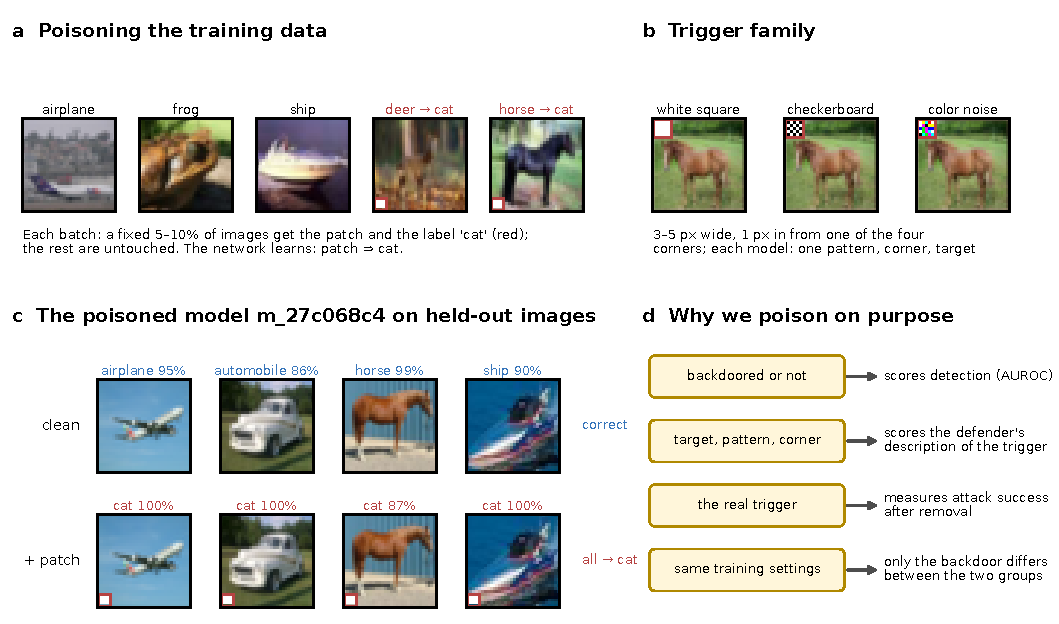
\includegraphics[width=\linewidth]{poisoning.pdf}
  \caption{\textbf{How the backdoored models are made.} (a) BadNets poisoning: in every training
  batch a fixed fraction of images get the trigger and the target label (here \emph{cat}). (b) The
  three trigger patterns. (c) Real predictions (softmax probability) of zoo model
  \texttt{m\_27c068c4} (white $3{\times}3$ patch, bottom-left, target \emph{cat}; patch outlined in
  red) on held-out test images. (d) Planting the backdoor ourselves gives a ground-truth answer for
  everything the defenders are asked.}
  \label{fig:poisoning}
\end{figure}

\subsection{Zoo construction}
Each model's training configuration is sampled from the same distribution whether or not it is
backdoored (Table~\ref{tab:hparams}); only backdoored models additionally sample a poison rate and a
trigger. Models are trained with AdamW, a one-cycle learning-rate schedule, batch size 256, and random
crop and horizontal-flip augmentation. Two disjoint zoos are trained with different random seeds: a
\textbf{meta-train zoo} of 80 models (40 backdoored), used only to fit the meta-classifier and to
calibrate the weight heuristic, and an \textbf{evaluation zoo} of 40 models (20 backdoored) on which
every reported number is computed. Each model gets a random identifier; its label, trigger and
configuration are written only to a separate key file from which no defender input is ever built.

\begin{table}[!htb]
  \centering
  \caption{\textbf{Sampled training configuration.} Values are drawn uniformly from each set,
  independently per model. The upper block is shared by clean and backdoored models.}
  \label{tab:hparams}
  \small
  \begin{tabular}{llc}
    \toprule
    Parameter & Values & Applies to \\
    \midrule
    Epochs & $\{20, 25, 30\}$ & all \\
    Peak learning rate & $\{3, 5, 8\} \times 10^{-3}$ & all \\
    Weight decay & $\{0,\ 10^{-4},\ 5 \times 10^{-4}\}$ & all \\
    Seed & random 31-bit integer & all \\
    \midrule
    Poison rate & $\{0.05, 0.08, 0.10\}$ & backdoored \\
    Trigger pattern & white square, checkerboard, colour noise & backdoored \\
    Trigger size & $\{3, 4, 5\}$ pixels & backdoored \\
    Trigger corner & top-left, top-right, bottom-left, bottom-right & backdoored \\
    Target class & $\{0, \dots, 9\}$ & backdoored \\
    \bottomrule
  \end{tabular}
\end{table}

\subsection{Data splits and metrics}
The 10{,}000 CIFAR-10 test images are split once. The first 1{,}000 are the \textbf{defender set}:
the only data any defence, including the LLM agent, may use. The remaining 9{,}000 are
\textbf{held out} for scoring. \emph{Clean accuracy} is top-1 accuracy on the held-out images.
\emph{Attack success rate} (ASR) is the fraction of held-out images whose true class is not the target
that the model assigns to the target once the real trigger is stamped. Detection is scored by AUROC of
each method's backdoor probability, by accuracy at threshold 0.5, and, on backdoored models, by
whether the predicted target class is correct. Uncertainty is reported as 95\% percentile bootstrap
intervals over models~\citep{efron1979bootstrap} (2{,}000 resamples).

% ============================================================================
\section{How an LLM inspects and edits weights}
\label{sec:llm}
An LLM cannot take a tensor as input; it reads text and images. The mechanism that lets it inspect a
network is therefore a \emph{serialisation} of the weights into a form it can read
(Section~\ref{sec:read}), and the mechanism that lets it change one is a \emph{tool}: a Python
sandbox in which the code it writes is executed against the weights (Section~\ref{sec:write}).

\subsection{Reading: weights as text or images, in one prompt}
\label{sec:read}
Figure~\ref{fig:read} shows the full path with the real input and output for one model. In the
\textbf{text view}, each tensor is quantised to integers $q \in [-99, 99]$ with one scale factor per
tensor ($w \approx q \cdot s$), so every weight takes one to three characters. Convolution weights are
written one output channel per line, with the nine values of each $3{\times}3$ kernel in reading
order; the classifier is written one class per line, with one value per conv3 channel. The whole
network is about 79{,}000 characters, or 64{,}000 tokens. In the \textbf{image view}, the same weights
are drawn as five plots: the conv1 filters as RGB patches and as separate R, G, B kernels, the conv2
and conv3 kernels as diverging heat-map mosaics, their per-kernel norms and biases, and the classifier
matrix (about 6{,}500 tokens). A third mode sends both.

The prompt also contains the architecture, the input normalisation, the class names and the threat
model: that about half the networks are backdoored, which patch patterns, sizes and corners are
possible, and that training settings carry no signal. The LLM cannot run code or the network. It
returns, in a fixed JSON schema, a probability that the network is backdoored, the most likely target
class, a guess at the pattern and corner, and a short statement of its evidence. This is directly
comparable to the weights-only baselines.

\begin{figure}[!htb]
  \centering
  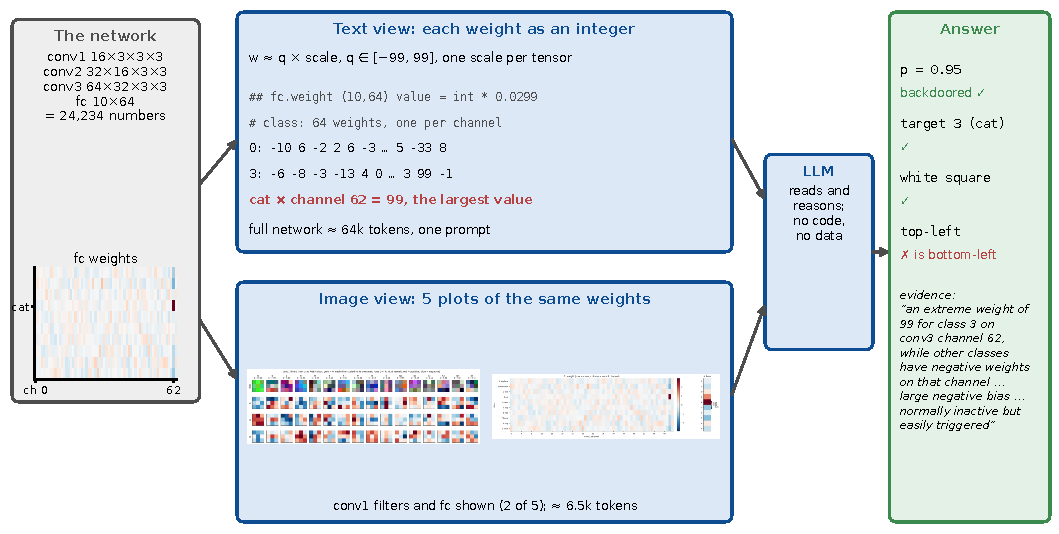
\includegraphics[width=\linewidth]{mechanism_read.pdf}
  \caption{\textbf{How an LLM reads a network} (detection task), with the real input and output for
  model \texttt{m\_27c068c4}. The weights are serialised as integers with one scale per tensor, or as
  five rendered plots, and sent in one prompt with the architecture and threat model. The LLM returns a
  probability, target, pattern, corner and evidence. Here Nemotron~3 Ultra points to conv3 channel 62
  feeding the \emph{cat} logit, which is the actual backdoor neuron (Section~\ref{sec:case}), and
  notes that the corner cannot be read from the weights.}
  \label{fig:read}
\end{figure}

\subsection{Writing: an agent in a metered Python sandbox}
\label{sec:write}
For removal, the LLM works as an agent (Figure~\ref{fig:agent}). It has one tool, \texttt{python},
which runs code in a persistent sandbox process and returns the printed output, any error, and any
figure the code passes to \texttt{show()}, which the LLM then sees as an image. The sandbox holds the
eight weight tensors \texttt{W}, which the agent may change freely, the 1{,}000 defender images and
their labels, and two functions that run the network: \texttt{forward(W, x)} returns logits and
\texttt{activations(W, x)} returns every layer's output. Each call costs one \emph{forward pass} of
up to 1{,}000 images, and the agent has 50 in total. When it is done, it calls \texttt{submit(W)}; the
last submitted weights are scored outside the sandbox with the real trigger, which the agent never
sees.

The agent is told that the network is backdoored and which kinds of trigger are possible, but not the
target, pattern or corner. The rules forbid gradients and optimisers, a home-made forward pass that
would bypass the meter, and file access. Every transcript is checked by an automatic audit for code
that breaks these rules; all 20 transcripts passed. The agent is free to look at weights, craft its
own test images (for example, clean images with candidate patches), and test edits before submitting.

\begin{figure}[!htb]
  \centering
  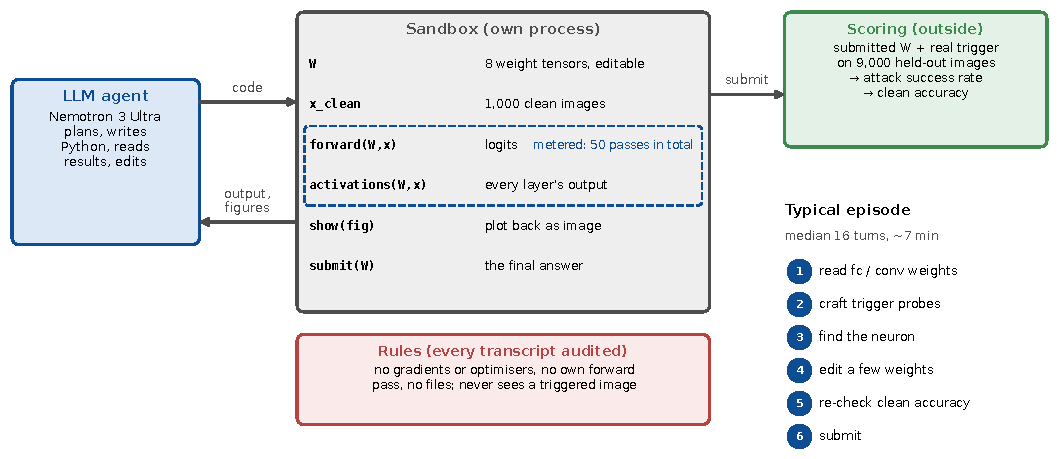
\includegraphics[width=\linewidth]{mechanism_agent.pdf}
  \caption{\textbf{How the LLM agent edits weights} (removal task). The agent sends Python code
  through a tool call; a persistent sandbox runs it and returns output, errors and figures. Running the
  network is metered (50 forward passes); gradients, a home-made forward pass and file access are
  forbidden and every transcript is audited. The last weights passed to \texttt{submit()} are scored
  outside the sandbox with the real trigger.}
  \label{fig:agent}
\end{figure}

\subsection{Models and runs}
Text-mode detection and the removal agent use \textbf{Nemotron~3 Ultra}, a reasoning model without
image input. The image and text+image modes use \textbf{Nemotron~3.5 Super VL}, which reads
images.\footnote{API model ids: \texttt{nvidia/nemotron-3-ultra-550b-a55b} and
\texttt{nvidia/nemotron-3.5-super-vl-120b-a12b}.} Both were called through NVIDIA's free API catalog with default sampling, at most
32{,}768 output tokens per call, and one run per model and mode. Table~\ref{tab:runs} summarises the
runs. The whole LLM study took about 440 requests and finished in under three hours of wall time.

\begin{table}[!htb]
  \centering
  \caption{\textbf{LLM runs.} Medians per model; ``turns'' is the number of LLM calls per model.
  Tokens are summed over all turns of a removal episode. ``No answer'': detection calls that ran out
  of output tokens while reasoning, or removal episodes with nothing submitted.}
  \label{tab:runs}
  \small
  \setlength{\tabcolsep}{4pt}
  \begin{tabular}{llcccccc}
    \toprule
    Experiment & LLM & Models & Turns & In tok. & Out tok. & Min. & No ans. \\
    \midrule
    \tabin{llm_runs_rows.tex}
    \bottomrule
  \end{tabular}
\end{table}

% ============================================================================
\section{Baselines}
\label{sec:methods}
\paragraph{Detection} (three methods, increasing access).
The \textbf{weight heuristic} (weights only, no training) takes the largest entry of the classifier
weight matrix divided by the standard deviation of all its entries, on the reasoning that a backdoor
must route a trigger feature to one class; the predicted target is the row holding it, and a
one-feature logistic regression fitted on the meta-train zoo turns the score into a probability. The
\textbf{meta-classifier} (weights and meta-train zoo) computes 16 permutation-invariant statistics per
layer plus four classifier-outlier features, 68 in total, and fits a standardised
$\ell_2$-regularised logistic regression ($C{=}0.3$) on the 80 meta-train models; it uses the
heuristic's target. \textbf{Neural Cleanse}~\citep{wang2019neuralcleanse} (weights, defender images
and gradients) optimises a mask and pattern per class with Adam (300 steps, learning rate 0.1, mask
$\ell_1$ penalty $10^{-2}$); the anomaly index of the smallest mask is mapped to a probability with a
logistic function centred on the standard threshold of 2, and the target is the class with the
smallest mask.

\paragraph{Removal} (four methods, defender set only, never a triggered image).
\textbf{Prune outlier} zeroes the conv3 channel feeding the largest standardised classifier weight.
\textbf{Fine-tune} trains all layers on the defender set (Adam, learning rate $10^{-3}$, 20 epochs,
batch 128, augmentation). \textbf{Fine-pruning}~\citep{liu2018fineprune} prunes conv3 channels in
order of mean activation on the defender set until defender accuracy drops by more than 3 points,
then fine-tunes with pruned channels held at zero. \textbf{NC unlearn}~\citep{wang2019neuralcleanse}
stamps Neural Cleanse's reversed trigger on 20\% of each batch with the \emph{true} labels and
fine-tunes. The three fine-tuning-based methods use gradients freely; the LLM agent may not.

% ============================================================================
\section{Results}
\label{sec:results}
\subsection{The zoo: strong, invisible backdoors}
Backdoors were implanted reliably: mean held-out ASR is 97.2\% in the meta-train zoo and 96.7\% in
the evaluation zoo, and no backdoored model falls below 85.7\% (Figure~\ref{fig:zoo},
Table~\ref{tab:zoo}). Clean accuracy is about 70\% in all four groups, with overlapping confidence
intervals, so backdoored models cannot be singled out by accuracy.

\begin{figure}[!htb]
  \centering
  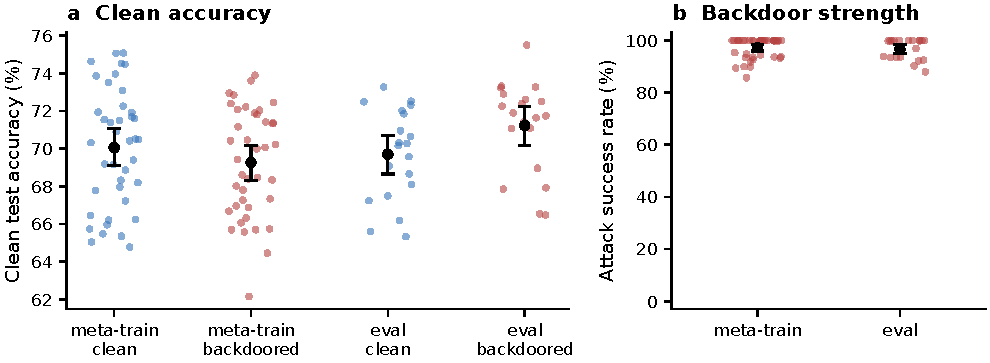
\includegraphics[width=0.86\linewidth]{zoo_summary.pdf}
  \caption{\textbf{Model zoo.} (a) Held-out clean accuracy for clean and backdoored models in each
  zoo. (b) Attack success rate of the backdoored models. Dots are models; black markers are means
  with 95\% bootstrap CIs.}
  \label{fig:zoo}
\end{figure}

\begin{table}[!htb]
  \centering
  \caption{\textbf{Zoo summary.} Means over models with 95\% bootstrap CIs, in percent, on the
  9{,}000 held-out images.}
  \label{tab:zoo}
  \small
  \begin{tabular}{llccc}
    \toprule
    Zoo & Group & $n$ & Clean accuracy (\%) & Attack success (\%) \\
    \midrule
    \tabin{zoo_rows.tex}
    \bottomrule
  \end{tabular}
\end{table}

\subsection{Detection: the LLM reads poorly}
The three baselines separate backdoored from clean models well (Figure~\ref{fig:detect}a,
Table~\ref{tab:detect}): the weights-only meta-classifier reaches AUROC 0.94, on par with Neural
Cleanse (0.92), and even the training-free weight heuristic reaches 0.87. The LLMs reach only
0.61--0.65 in all three input modes, and the lower ends of their confidence intervals lie below 0.5.
At the 0.5 threshold they are right on 50--57\% of models, against 80--82\% for the baselines.

\begin{figure}[!htb]
  \centering
  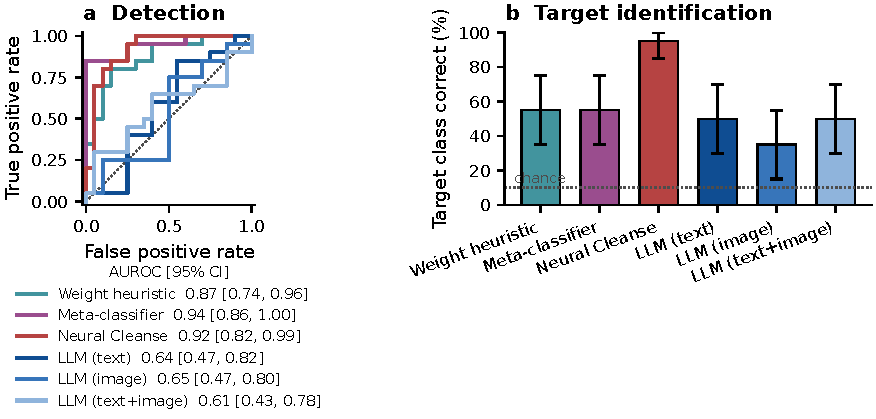
\includegraphics[width=0.84\linewidth]{detect_baselines.pdf}
  \caption{\textbf{Detection on the evaluation zoo} (40 models, 20 backdoored). (a) ROC curves;
  AUROC with 95\% bootstrap CI in the legend. (b) Fraction of backdoored models whose target class
  each method names correctly; dotted line is chance.}
  \label{fig:detect}
\end{figure}

\begin{table}[!htb]
  \centering
  \caption{\textbf{Detection results}, evaluation zoo. Brackets are 95\% bootstrap CIs over models.
  Target accuracy is over the 20 backdoored models. Unanswered LLM calls count as $p{=}0.5$ with a
  wrong target.}
  \label{tab:detect}
  \small
  \begin{tabular}{llccc}
    \toprule
    Method & Input & AUROC & Accuracy @0.5 (\%) & Target correct (\%) \\
    \midrule
    \tabin{detect_rows.tex}
    \bottomrule
  \end{tabular}
\end{table}

Figure~\ref{fig:detect-llm} shows why. The LLM rarely says ``clean'': in text mode it gives 17 of the
20 clean models a probability above 0.5 (mean 0.78, against 0.87 for backdoored models), and the
other two modes give mean probabilities of 0.54--0.69 with similarly small gaps between clean and
backdoored models. Its stated probabilities therefore carry
little ranking information. When it names a target class, it does better than chance (50\% in text
mode against 10\% chance) but no better than the weight heuristic: the text-mode LLM is right on
exactly 10 models, and the heuristic is right on all ten of them. The LLM appears to find the same
signal, an outlying classifier weight, without adding to it. Trigger pattern guesses are near chance
(40--45\% against 33\%), and corner guesses are at or below chance (15--30\% against 25\%). The corner
result is expected and the LLM often says so itself (Figure~\ref{fig:read}): convolutions share
weights across positions and global average pooling discards position, so the corner leaves little
trace in the weights.

\begin{figure}[!htb]
  \centering
  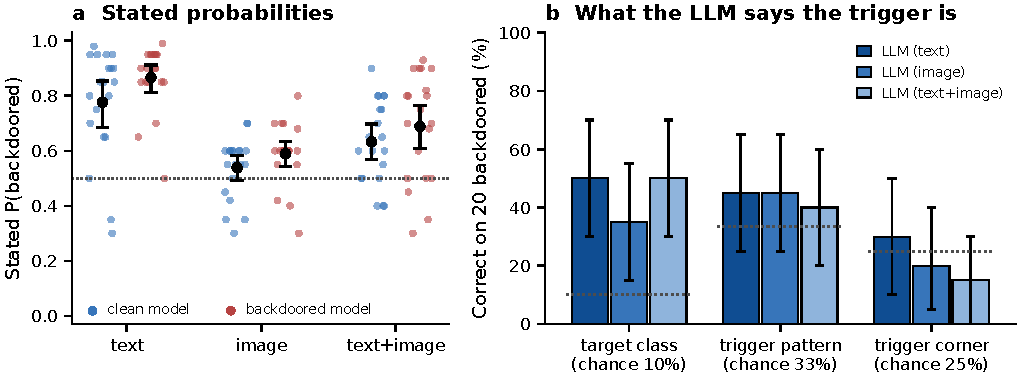
\includegraphics[width=0.92\linewidth]{detect_llm.pdf}
  \caption{\textbf{The LLM detectors in detail.} (a) Backdoor probability stated for each clean
  (blue) and backdoored (red) model, by input mode; black markers are means with 95\% bootstrap CIs.
  (b) Fraction of the 20 backdoored models for which the LLM names the true target, pattern and
  corner; dotted lines are chance.}
  \label{fig:detect-llm}
\end{figure}

Figure~\ref{fig:mechanism} shows what the baselines rely on. Backdoored models tend to carry an
outlying classifier weight (panel a: mean 5.35 standard deviations against 3.35 for clean models),
but in 9 of the 20 backdoored models the target's largest weight is not the largest overall, so any
method that takes the argmax names the wrong class. Neural Cleanse instead measures what each class
\emph{does}: in 19 of 20 backdoored models the true target needs the smallest mask of all classes
(panel c). Reading weights reveals that a backdoor is present far more reliably than where it points.

\begin{figure}[!htb]
  \centering
  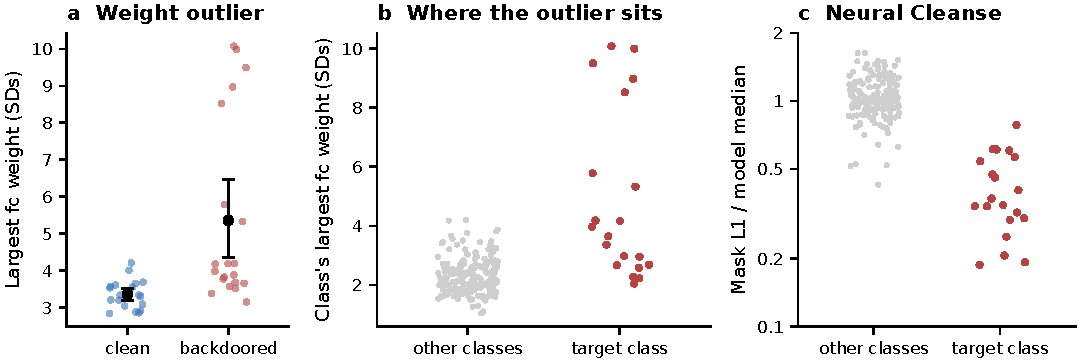
\includegraphics[width=0.96\linewidth]{detect_mechanism.pdf}
  \caption{\textbf{What the baselines see.} (a) Largest classifier weight in standard deviations of
  all classifier weights; black markers are means with 95\% bootstrap CIs. (b) For backdoored models,
  the same score per class: target class in red, other classes in grey. (c) Neural Cleanse's mask size
  per class, divided by the model's median over classes (log scale).}
  \label{fig:mechanism}
\end{figure}

\subsection{Removal: the LLM agent writes well}
Removal without triggered data is hard for every method (Figure~\ref{fig:remove},
Table~\ref{tab:remove}). Fine-tuning on 1{,}000 clean images barely touches the backdoor (ASR 94.5\%),
and pruning the outlier channel helps only sometimes (79.1\%). Fine-pruning and NC unlearn are the
strongest baselines, at 62.2\% and 42.8\% mean ASR, and each brings 5 of 20 models below 20\%.

The LLM agent reaches a mean ASR of 51.9\%, between the two strongest baselines, and brings
\textbf{6 of 20} models below 20\%, the most of any method. Its mean clean accuracy is 69.5\%, a drop
of 1.7 points from the original models, similar to the baselines' drops of 0.7--2.8 points. Every
episode ended with weights submitted, and the agent stopped on its own each time.

\begin{figure}[!htb]
  \centering
  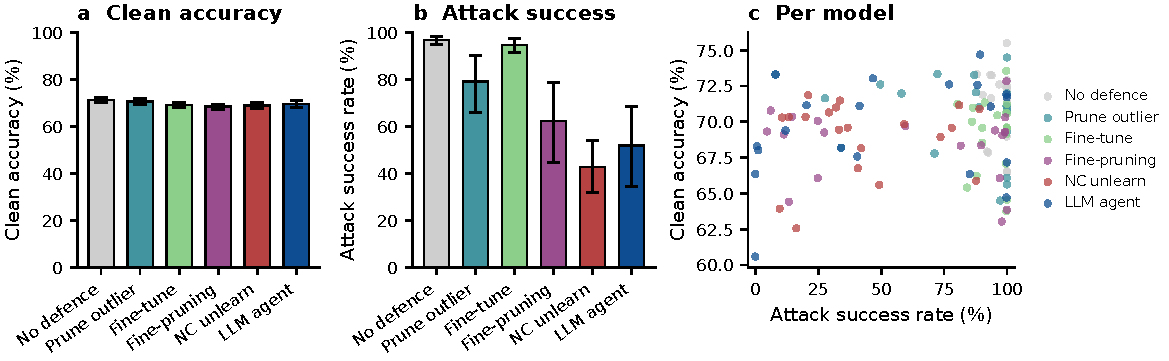
\includegraphics[width=\linewidth]{remove_baselines.pdf}
  \caption{\textbf{Removal on the 20 backdoored evaluation models.} (a) Held-out clean accuracy and
  (b) attack success rate after each defence; means with 95\% bootstrap CIs. (c) Each dot is one
  model after one defence; the ideal is the top-left corner.}
  \label{fig:remove}
\end{figure}

\begin{table}[!htb]
  \centering
  \caption{\textbf{Removal results}, 20 backdoored evaluation models. Means with 95\% bootstrap CIs
  on the held-out images. The last column counts models brought below 20\% ASR.}
  \label{tab:remove}
  \small
  \begin{tabular}{lccc}
    \toprule
    Defence & Clean accuracy (\%) & Attack success (\%) & ASR $<$ 20\% \\
    \midrule
    \tabin{remove_rows.tex}
    \bottomrule
  \end{tabular}
\end{table}

The average hides an all-or-nothing pattern (Figure~\ref{fig:remove-llm}a). On six models the agent
removes the backdoor almost completely (ASR 0--12\%); on eight it leaves more than 80\% in place;
the rest are partial. Its edits are tiny: a median of 6 of the 24{,}234 weights, never more than 40
(panel c). Per model, the agent beats NC unlearn on 11 of 20 networks in this run (panel b; 7 of 20
when each model's ASR is averaged over three runs, Section~\ref{sec:repeats}), and the two fail on
different ones: taking the better of the two for each network would give a mean ASR of 27.8\% and
9 of 20 networks below 20\%. This combination is an oracle, since a defender cannot see the ASR, but it
shows how complementary the two are.

\begin{figure}[!htb]
  \centering
  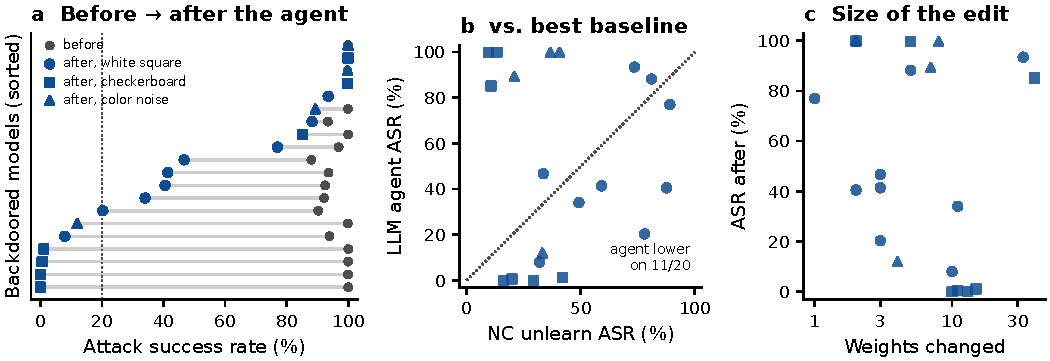
\includegraphics[width=\linewidth]{remove_llm.pdf}
  \caption{\textbf{The LLM removal agent in detail.} (a) Held-out ASR before (grey) and after (blue)
  the agent's edit, one row per model, sorted; marker shape is the trigger pattern. (b) Per model,
  the agent's ASR against NC unlearn's; points below the diagonal favour the agent. (c) Number of
  weights changed (log scale) against the resulting ASR.}
  \label{fig:remove-llm}
\end{figure}

The trigger pattern matters for every method (Figure~\ref{fig:bytrigger}, Table~\ref{tab:pattern}).
Pruning-based baselines handle white squares best, NC unlearn handles checkerboard and colour noise
best. The agent's results are split within patterns: on checkerboards it removes four backdoors
completely (ASR at most 1.2\%) and leaves three at 85--100\%. These four removals used its largest
successful edits (10--15 weights) and cost the most clean accuracy (3.4--6.5 points), while its edits
on white squares left accuracy almost unchanged.

\begin{figure}[!htb]
  \centering
  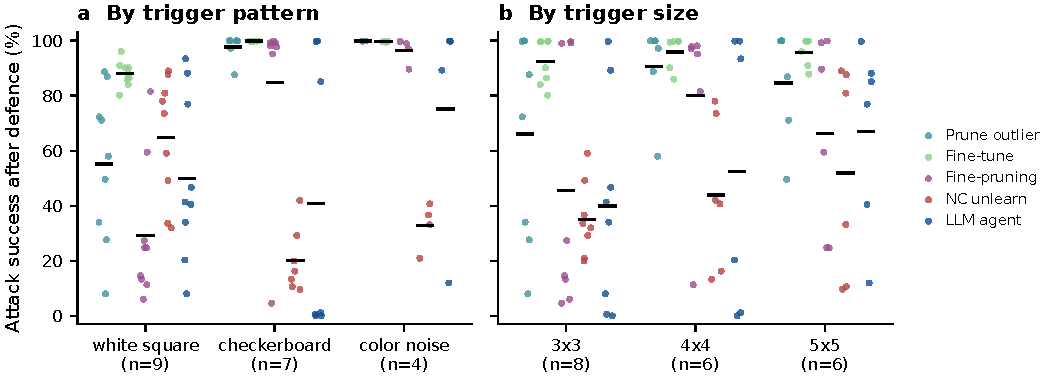
\includegraphics[width=0.96\linewidth]{remove_by_trigger.pdf}
  \caption{\textbf{Removal by trigger type.} ASR after each defence, split by (a) trigger pattern and
  (b) trigger size; $n$ counts backdoored evaluation models per group. Dots are models, black bars
  group means. Groups are small; the panels are descriptive, not significance tests.}
  \label{fig:bytrigger}
\end{figure}

\begin{table}[!htb]
  \centering
  \caption{\textbf{Mean attack success (\%) after each defence, by trigger pattern.} Bold marks the
  best defence per pattern.}
  \label{tab:pattern}
  \small
  \begin{tabular}{lccccccc}
    \toprule
    Pattern & $n$ & No defence & Prune & Fine-tune & Fine-prune & NC unlearn & LLM agent \\
    \midrule
    \tabin{pattern_rows.tex}
    \bottomrule
  \end{tabular}
\end{table}

\subsection{Inside one episode: finding and switching off the backdoor neuron}
\label{sec:case}
Figure~\ref{fig:case} follows the agent on model \texttt{m\_27c068c4} (white $3{\times}3$ patch,
bottom-left, target \emph{cat}), using its transcript. In its first five turns, using a single
forward pass to check clean accuracy, the agent reads the weights: it finds that conv3 channel 62 sends
the largest classifier weight of the network into \emph{cat} (2.96), with negative weights into most
other classes (panel a), and that the channel also has the largest conv3 kernel norm and a strongly
negative bias ($-0.96$): a feature that is normally off. It then tests the hypothesis with patches it
builds itself. A white $3{\times}3$ patch in the bottom-left corner drives channel 62 to 4.6 on a clean
image (7.5 on a blank one), while clean images leave it near zero (panel b shows the same contrast
measured with the real trigger), and its own estimate of the
attack success on 50 patched images is 92\%. It tries the edit on a copy of the weights, setting the
ten classifier weights leaving channel 62 to zero, and checks that none of the 1{,}000 clean
predictions changes. It sweeps 36 candidate triggers (four corners, three patterns, three sizes) on
the edited copy, applies the edit, and submits. On held-out data the ASR falls from 94\% to 8\% and
clean accuracy is unchanged (73.2\% to 73.3\%; panel d).

The episode is a small-scale version of a mechanistic interpretability workflow: form a hypothesis
from the weights, confirm it with a controlled experiment, make a minimal causal edit, and verify it.
It also shows the agent's main limitation. The budget is spent largely on confirming the hypothesis
and checking side effects (panel c); every one of the 20 episodes used all 50 forward passes. When
the backdoor is not carried by a single outstanding channel, the same workflow finds nothing to
switch off, or switches off the wrong channel.

\begin{figure}[!htb]
  \centering
  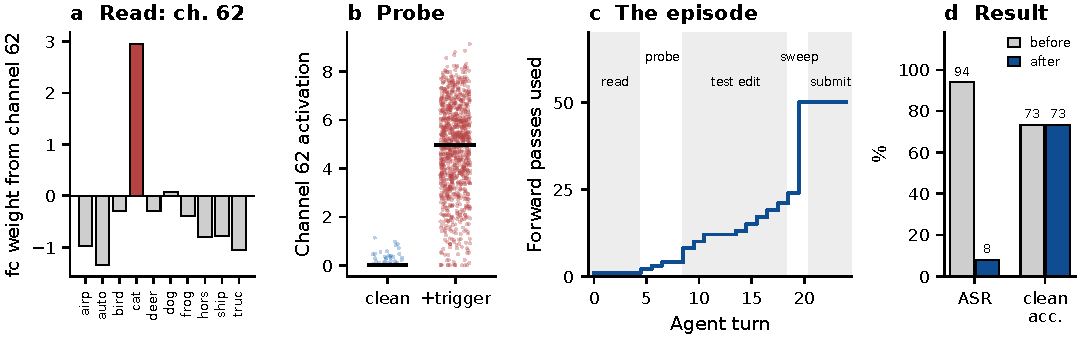
\includegraphics[width=\linewidth]{case_study.pdf}
  \caption{\textbf{One removal episode} (model \texttt{m\_27c068c4}). (a) Classifier weights leaving
  conv3 channel 62: large and positive into \emph{cat}. (b) The channel's activation on the 1{,}000
  defender images, clean and with the real trigger (medians as black bars). (c) Forward passes used by
  turn, with phases summarised from the transcript. (d) Held-out ASR and clean accuracy before and
  after the edit, which zeroed the ten classifier weights of channel 62.}
  \label{fig:case}
\end{figure}

\subsection{Ablations: does the agent read the weights or probe the network?}
\label{sec:ablation}
The agent can learn about a network in two ways: by reading the weights, or by running the network on
inputs it designs and watching predictions and activations (probing). Either route can end in the same
edit, so the main experiment cannot tell which one does the work. We therefore reran removal on the same
20 models with the same LLM and prompt, removing one route at a time.
\emph{Weights only}: the agent reads and edits every weight but cannot run the network and has no
images. \emph{Probing only}: the agent runs the network (50 forward passes, activations included) and
edits weights by position, for example ``multiply column 62 of \texttt{fc.weight} by 0'', but cannot
read any weight value; the weights sit behind a handle that exposes only shapes, and the rules forbid
solving for weights from activations. A third, \emph{random edit}, uses no LLM: it takes the full
agent's edit on each model and applies it at random positions of the same tensors (10 draws). The audit
flagged 3 probing-only transcripts; on inspection every hit was in a comment or a shape query, and no
transcript in any condition broke a rule.

\begin{table}[!htb]
  \centering
  \caption{\textbf{Removal ablations}, 20 backdoored evaluation models, Nemotron~3 Ultra. Means with
  95\% bootstrap CIs on held-out images, from run 1. ``ASR $<$ 20\%'' counts models brought below 20\%
  ASR with a working network (clean accuracy at least 20\%). The last column averages each model's ASR
  over three independent runs (Section~\ref{sec:repeats}).}
  \label{tab:ablation}
  \small
  \setlength{\tabcolsep}{4pt}
  \begin{tabular}{lcccccc}
    \toprule
    Condition & Reads & Runs & Clean acc. (\%) & ASR (\%) & ASR $<$ 20\% & ASR, 3 runs (\%) \\
    \midrule
    \tabin{ablation_rows.tex}
    \bottomrule
  \end{tabular}
\end{table}

\begin{figure}[!htb]
  \centering
  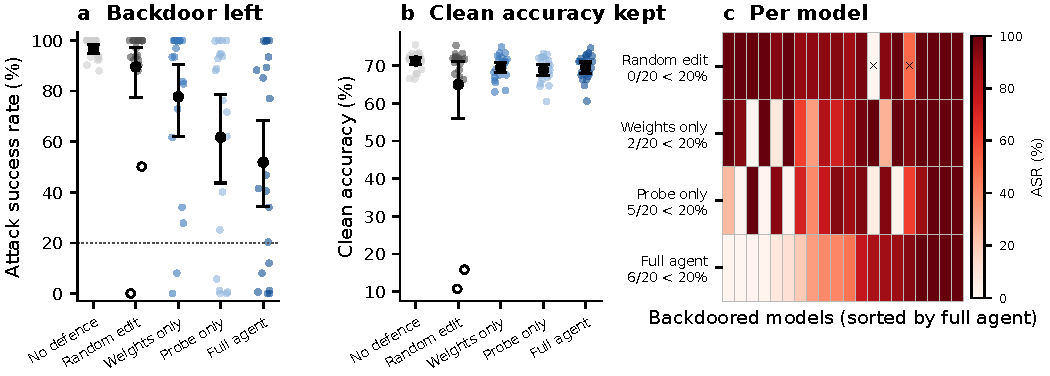
\includegraphics[width=\linewidth]{ablation.pdf}
  \caption{\textbf{Where the agent's success comes from.} (a) Held-out ASR and (b) clean accuracy per
  condition; dots are models, black markers means with 95\% bootstrap CIs; hollow circles are random
  edits that broke the network (clean accuracy below 20\%). (c) ASR per model and condition, models
  sorted by the full agent; $\times$ marks a broken network.}
  \label{fig:ablation}
\end{figure}

Table~\ref{tab:ablation} and Figure~\ref{fig:ablation} give the answer: \emph{both routes matter, and
probing matters more.} The ordering is random edit (89.5\% mean ASR), weights only (77.7\%), probing
only (61.7\%), full agent (51.9\%). Paired by model, the full agent beats weights only clearly (mean
difference $-25.8$ points, 95\% CI $[-43.5, -8.1]$; lower by more than 5 points on 11 models, higher on 1; Wilcoxon signed-rank
$p=0.009$), but in this single run it is not separable from probing only ($-9.9$ points, CI
$[-28.9, 9.9]$, $p=0.25$); averaged over three runs it is (below).
Probing only beats random edits ($p=0.03$); weights only does not resolve from them ($p=0.14$). The
random-edit control also shows that the full agent's edits work because of \emph{where} they land, not
because they are small: moved elsewhere, the same edits leave 89.5\% ASR, against 51.9\% in place
($p=0.002$).

The per-model view is more informative than the means. Reading alone solves 2 models, and they are
telling: on \texttt{m\_27c068c4} (the case study) the weights-only agent, which never ran the network,
submitted \emph{exactly} the full agent's edit, zeroing the ten classifier weights of channel 62
(ASR 8\%), while the probing-only agent, unable to see that channel 62 stands out, scaled down the whole
\emph{cat} row and left the backdoor in place (93\%). On \texttt{m\_47995f26} the weights-only edit shares
8 of its 9 weights with the full agent's. Probing alone solves 5 models, three of them also solved by the
full agent. Five of the full agent's six successes are thus reached by one route alone, two by reading and
three by probing: some backdoors announce themselves in a weight that stands out, others are found only
by experiment. Neither route alone reaches the full agent's count.

\subsection{Repeat runs: how much does one run tell us?}
\label{sec:repeats}
LLM agents sample their actions, so one run per model may be luck. We repeated all three agent
conditions twice more on the same 20 models with the same LLM and prompts: 120 further episodes, 180
in total (Figure~\ref{fig:repeats}). The averages are stable: mean ASR per run is 44.6--54.9\% for the
full agent, 53.5--66.0\% for probing only and 73.1--80.6\% for weights only, and the ordering is the same
in every run. Individual models are not stable. For the full agent, a model's ASR differs by a median of
60 points between its best and worst run, and 11 of the 20 models swing by more than 50 points. The
agent removes the backdoor (ASR below 20\%) on 5--6 models per run, but on 11 different models across
the three runs, and on only one in all three. Probing only behaves the same way (4--6 per run, 12
different models, none in all three). Weights only is steadier (median spread 2 points) because it usually
changes little.

Averaging each model over its three runs gives tighter comparisons (last column of
Table~\ref{tab:ablation}). The full agent (50.4\%, CI $[40.3, 59.7]$) now beats probing only (60.4\%,
CI $[50.2, 69.5]$) clearly: paired difference $-10.0$ points, CI $[-16.5, -3.4]$, Wilcoxon $p=0.009$.
Reading the weights therefore adds to probing, not only on the two models where it is enough on its own.
Probing only beats weights only by 16.7 points ($p=0.053$). Against NC unlearn (42.8\%), the run-averaged
agent is not resolved ($p=0.35$; lower on 7 of 20 models). In 180 episodes the audit found one genuine rule
break: in a repeat of the full condition, after using all 50 passes, the agent wrote its own forward pass
to check clean accuracy on the 1{,}000 defender images. That episode left the backdoor intact (ASR
99.9\%), so the results do not change whether it is counted or not. Every other flag was a comment, a
shape query, or an \texttt{import sys} used to list variables.

\begin{figure}[!htb]
  \centering
  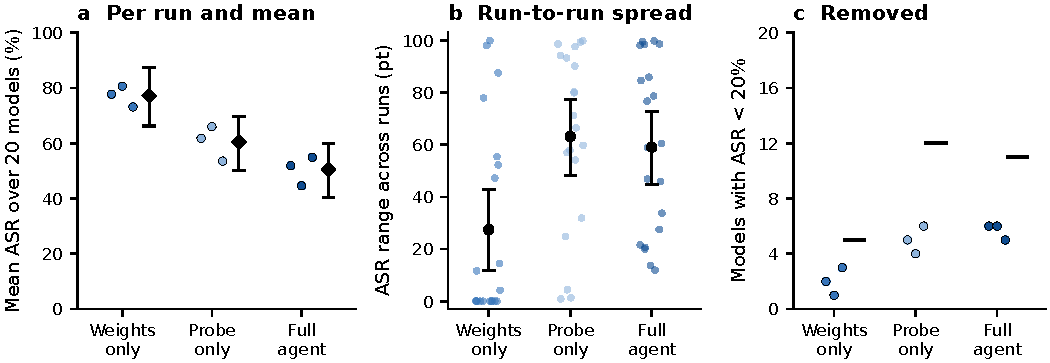
\includegraphics[width=\linewidth]{repeats.pdf}
  \caption{\textbf{Run-to-run variation}, three independent runs of each agent condition on the same 20
  models. (a) Mean ASR of each run (dots) and the mean over runs with a 95\% bootstrap CI over models
  (diamond). (b) Per model, ASR range across runs (best minus worst); black markers are means with 95\%
  CIs. (c) Models brought below 20\% ASR in each run (dots) and in at least one run (bar).}
  \label{fig:repeats}
\end{figure}

\subsection{Best of three: can a defender pick the good run?}
\label{sec:bestofk}
Since the agent often fixes a model in one run and not in another, a defender could run it several times
and keep the best repair, if it can tell which one that is without the real trigger. We tested a check
the defender can run, mirroring what the agent itself does: stamp 60 candidate triggers from the family
the agent was told about (three patterns, sizes 3--5, four corners, three random seeds for colour noise,
since the real seed is unknown) on the 1{,}000 defender images, and take the largest share of images any
candidate sends to one class as the \emph{estimated} ASR. We fixed the selection rule before looking at
outcomes: among a model's three runs whose defender clean accuracy is at most 5 points below the
original's, keep the one with the lowest estimated ASR. Selection uses no held-out data.

\begin{figure}[!htb]
  \centering
  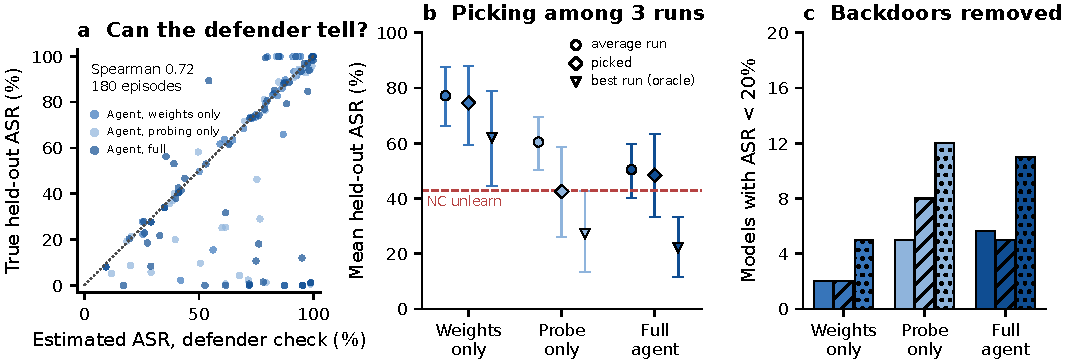
\includegraphics[width=\linewidth]{best_of_k.pdf}
  \caption{\textbf{Picking among three runs without the real trigger.} (a) Defender's estimated ASR
  (60 candidate triggers on its 1{,}000 clean images) against the true held-out ASR, for all 180
  episodes. (b) Mean held-out ASR of an average run, of the run the defender picks, and of the best run
  (oracle); 95\% bootstrap CIs over 20 models; dashed line is NC unlearn. (c) Models below 20\% ASR:
  average per run (plain), picked (hatched), oracle (dotted).}
  \label{fig:bestofk}
\end{figure}

The estimate tracks the truth reasonably well (Spearman 0.72 over 180 episodes; Figure~\ref{fig:bestofk}a),
but it errs in one direction: on some networks whose real backdoor is gone, a candidate patch still
pushes many images to one class, so the check reports a high ASR. With the pre-registered rule, picking
helps the probing-only agent substantially (mean ASR 60.4\% for an average run, 42.5\% picked, $p=0.009$;
8 of 20 models below 20\%, against 5 per run), but barely helps the full agent (50.4\% to 48.4\%,
$p=0.57$; 5 of 20), against an oracle of 22.3\% with 11 of 20. The reason is the accuracy filter, not the
estimate: in 8 of the 11 models where it missed the full agent's best run, that run cost slightly more
than 5 points of defender clean accuracy and was excluded. As an \emph{exploratory} check, chosen after
seeing this, relaxing the filter to 8 points or more lowers the picked full agent to 33\% mean ASR with
8 of 20 models below 20\% ($p=0.006$ against an average run), below NC unlearn's 42.8\%, at a cost of
about one point of held-out clean accuracy. That threshold needs confirming on fresh models before it
can be trusted, but it suggests that much of the agent's run-to-run variance can be recovered by a
cheap check that needs no knowledge of the real trigger.

% ============================================================================
\section{Discussion}
\paragraph{Why reading fails and writing works.}
The two tasks differ in what the LLM can do with its reasoning. In detection, it must compare
thousands of numbers across a 64{,}000-token prompt without computing anything: no means, no standard
deviations, no ranking. A one-line statistic does this exactly; the LLM approximates it by eye, finds
it when it is large (the cases where it names the right target coincide with the heuristic's), and
otherwise falls back on its prior that backdoors are common, which inflates its probabilities on clean
models. In removal, the same model can compute statistics in code, run controlled experiments, and see
their results. The hard part of reading, comparing many numbers, becomes a one-line computation, and
what remains is forming and testing hypotheses, which the LLM does well.

\paragraph{Reading and probing are complementary.}
The ablations (Section~\ref{sec:ablation}) refine this picture. Most of the agent's removal power comes
from probing: designing candidate triggers and watching the network respond, a black-box search the LLM
runs well. Reading the weights still contributes: averaged over three runs, the full agent beats the
probing-only agent by 10 points ($p=0.009$). Without any forward pass the agent removed two
backdoors, with the same or nearly the same edit as the full agent, and on one of them (the case study)
the probing agent, which could not see that one channel stands out, missed that edit. The full agent does
best, consistent with each route covering cases the other misses: the weights suggest where to look, and
experiments decide.

\paragraph{What the agent adds.}
The agent's repairs are targeted: it edits a median of six weights, while the gradient-based baselines
change every weight in the network. This keeps clean accuracy intact when the target neuron is purely
a trigger detector, and it makes the repair explainable: each submission comes with the neuron it
blames and the evidence. The agent also succeeds on networks where the best baseline fails, and vice
versa. Its main weakness is consistency: the same model is repaired in one run and untouched in the next,
so a practical tool would run the agent several times and keep a repair it can verify
(Section~\ref{sec:bestofk}). A practical defence could also combine the agent with classical repairs,
with the agent diagnosing the trigger and choosing or calling one.

\paragraph{Limitations.}
The evaluation zoo has 40 models (20 backdoored), so confidence intervals are wide; differences such as
50.4\% versus 42.8\% mean ASR are not statistically resolved. Detection and the image modes were run
once per model. Removal was run three times per condition, which shows large run-to-run variation per
model (Section~\ref{sec:repeats}); per-model results from a single run should not be over-read. Detection modes used two different LLMs,
because only one reads images, so the comparison between text and image modes is confounded with the
model. Seven detection calls produced no answer because the LLM exhausted its output budget while
reasoning; they are counted as uninformative. All networks share one small architecture without batch
normalisation, and only patch-based BadNets attacks are studied, among the easiest backdoors to find.
The agent was told that each network in the removal task is backdoored. The audit of rule violations is
pattern-based and cannot exclude every indirect workaround; it found one rule break in 180 removal
episodes, which did not affect the result, and every flagged transcript was read in full.

% ============================================================================
\section{Future work}
\begin{enumerate}[leftmargin=*]
  \item \textbf{Let the reader compute.} Allow code in detection (a weights-only sandbox with no
    forward passes) to test whether the LLM's weak detection comes from reading without computing.
  \item \textbf{Combine the agent with classical repairs.} Give the agent Neural Cleanse, fine-pruning
    and unlearning as tools and let it choose from its own diagnosis, approaching the oracle
    combination (27.8\% mean ASR) without knowing the ASR.
  \item \textbf{Vary the budget and the models.} The ablations fix the two ends (0 and 50 forward
    passes); intermediate budgets (5, 10, 20) would show how many experiments reading saves. Confirm
    the best-of-$k$ selection rule, including its accuracy threshold, on a fresh zoo, and compare stronger
    frontier models with the open models used here.
  \item \textbf{Harder attacks and larger networks.} Blended and warping triggers, clean-label
    poisoning, multiple targets, attacks designed to hide from weight statistics, and architectures
    with batch normalisation and residual connections, where single weights are harder to read.
  \item \textbf{Faithfulness of explanations.} Check whether the neuron the agent blames actually
    carries the backdoor by ablating exactly what it names, across all models.
  \item \textbf{Scale the zoo} for tighter intervals and formal tests between methods.
\end{enumerate}

% ============================================================================
\section{Conclusion}
We built a controlled testbed for auditing neural networks through their weights and used it to test
whether LLMs can detect and remove backdoors. As readers, the LLMs tested here are weak: given every
weight as text or images and no way to compute, they detect backdoors only slightly better than chance
and find the target class only when a simple weight statistic does. As writers, they are competitive:
an LLM agent with a Python sandbox, a small forward-pass budget and no gradients finds the backdoor
neuron by its own experiments, removes the backdoor with a handful of weight edits, and succeeds on
networks where the best classical defence fails. Ablations show that most of this comes from
probing the network, but reading the weights adds to it: over three repeated runs, the full agent
beats a probing-only agent by 10 points of ASR, and reading alone solves cases that probing misses.
Individual runs vary a great deal, so repeated runs, not single episodes, are the right unit of
evaluation for such agents, and a simple trigger check lets a defender recover part of that variance by
keeping the best of several runs. Weight-space auditing by LLMs works best when the LLM can test its hypotheses, not
when it must judge by reading alone.

% ============================================================================
\appendix
\section{Reproducibility}
All code, the trained zoo, every LLM answer and transcript, and every figure are available at
\url{https://github.com/yukteswar23/backdoor-ws}. Figures and tables are generated from saved results
and can be rebuilt without retraining or new API calls.
\begin{center}
\small
\begin{tabular}{ll}
  \toprule
  Step & Command \\
  \midrule
  Build the dataset file & \texttt{python -m wsp\_vision.prepare\_data} \\
  Train both zoos (resumable) & \texttt{bash run\_zoo.sh} \\
  Baselines, then figures & \texttt{bash run\_baselines.sh} \\
  LLM experiments, audit, scoring & \texttt{NVIDIA\_API\_KEY=\dots\ bash run\_nvidia.sh} \\
  Removal ablations & \texttt{NVIDIA\_API\_KEY=\dots\ bash run\_ablation.sh} \\
  Repeat runs (2 and 3) & \texttt{NVIDIA\_API\_KEY=\dots\ bash run\_repeats.sh} \\
  Best-of-3 selection (no API) & \texttt{python -m wsp\_vision.agent.select\_runs} \\
  Figures and diagrams & \texttt{python -m wsp\_vision.plots.\{figures,llm\_figures,diagrams\}} \\
  This PDF (tables included) & \texttt{bash report/build.sh} \\
  \bottomrule
\end{tabular}
\end{center}
\noindent\textbf{Compute.} One NVIDIA GeForce RTX 2050 laptop GPU. Training takes about 45\,s per model
(about 1.5\,h for 120 models); Neural Cleanse takes about 97\,s per model; the full baseline suite took
1.6\,h. The LLM runs used NVIDIA's free API catalog, which is rate-limited (in our measurement, a burst
of about 30 requests was accepted within seconds before further requests were refused); with three removal episodes and up to seven detection calls in parallel, all LLM
experiments finished in under three hours. The two LLM ablations took a further 1.5\,h (probing only
about 2.4\,min and weights only about 10\,min per model, median), with scoring on the CPU. The two
repeat runs (120 episodes) took 6.3\,h, slowed by API overload (HTTP 503) during the second.

\section{Prompt summary}
\textbf{Detection} (system prompt, abridged): the LLM is told it audits small CIFAR-10 classifiers for
hidden backdoors using only their weights; it receives the architecture, normalisation and classes; it
is told that about half the networks are backdoored with a 3--5 pixel white-square, checkerboard or
colour-noise patch one pixel from a corner, relabelled to one target, and that training settings were
randomised identically for both groups. It must give a calibrated probability, a target class (always),
a pattern and corner (always, saying in the evidence if they cannot be read), and short evidence.
\textbf{Removal} (system prompt, abridged): the LLM is told that the network \emph{is} backdoored, the
trigger family, the sandbox contents and rules listed in Section~\ref{sec:write}, that it is scored on
held-out images by attack success and clean accuracy, and that it should work step by step, call
\texttt{submit(W)}, and end with a summary of what it changed and why. The full prompts are in
\texttt{wsp\_vision/agent/detect.py} and \texttt{remove.py}.

% ============================================================================
\begin{thebibliography}{99}
\small
\bibitem[Bills et~al.(2023)]{bills2023explain}
S.~Bills, N.~Cammarata, D.~Mossing, H.~Tillman, L.~Gao, G.~Goh, I.~Sutskever, J.~Leike, J.~Wu, and
W.~Saunders.
\newblock Language models can explain neurons in language models.
\newblock OpenAI, 2023.

\bibitem[Chen et~al.(2017)]{chen2017targeted}
X.~Chen, C.~Liu, B.~Li, K.~Lu, and D.~Song.
\newblock Targeted backdoor attacks on deep learning systems using data poisoning.
\newblock \emph{arXiv preprint arXiv:1712.05526}, 2017.

\bibitem[Efron(1979)]{efron1979bootstrap}
B.~Efron.
\newblock Bootstrap methods: another look at the jackknife.
\newblock \emph{The Annals of Statistics}, 7(1):1--26, 1979.

\bibitem[Gu et~al.(2017)]{gu2017badnets}
T.~Gu, B.~Dolan-Gavitt, and S.~Garg.
\newblock {BadNets}: Identifying vulnerabilities in the machine learning model supply chain.
\newblock \emph{arXiv preprint arXiv:1708.06733}, 2017.

\bibitem[Krizhevsky(2009)]{krizhevsky2009cifar}
A.~Krizhevsky.
\newblock Learning multiple layers of features from tiny images.
\newblock Technical report, University of Toronto, 2009.

\bibitem[Liu et~al.(2018)]{liu2018fineprune}
K.~Liu, B.~Dolan-Gavitt, and S.~Garg.
\newblock Fine-pruning: Defending against backdooring attacks on deep neural networks.
\newblock In \emph{Research in Attacks, Intrusions, and Defenses (RAID)}, 2018.

\bibitem[Navon et~al.(2023)]{navon2023equivariant}
A.~Navon, A.~Shamsian, I.~Achituve, E.~Fetaya, G.~Chechik, and H.~Maron.
\newblock Equivariant architectures for learning in deep weight spaces.
\newblock In \emph{International Conference on Machine Learning (ICML)}, 2023.

\bibitem[NVIDIA(2026)]{nvidia2026catalog}
NVIDIA.
\newblock NVIDIA API catalog.
\newblock \url{https://build.nvidia.com}, accessed November 2026.

\bibitem[Schick et~al.(2023)]{schick2023toolformer}
T.~Schick, J.~Dwivedi-Yu, R.~Dess{\`i}, R.~Raileanu, M.~Lomeli, L.~Zettlemoyer, N.~Cancedda, and
T.~Scialom.
\newblock Toolformer: Language models can teach themselves to use tools.
\newblock In \emph{Advances in Neural Information Processing Systems (NeurIPS)}, 2023.

\bibitem[Sch{\"u}rholt et~al.(2022)]{schurholt2022modelzoos}
K.~Sch{\"u}rholt, D.~Taskiran, B.~Knyazev, X.~Gir{\'o}-i-Nieto, and D.~Borth.
\newblock Model zoos: A dataset of diverse populations of neural network models.
\newblock In \emph{NeurIPS Datasets and Benchmarks Track}, 2022.

\bibitem[Tran et~al.(2018)]{tran2018spectral}
B.~Tran, J.~Li, and A.~Madry.
\newblock Spectral signatures in backdoor attacks.
\newblock In \emph{Advances in Neural Information Processing Systems (NeurIPS)}, 2018.

\bibitem[Unterthiner et~al.(2020)]{unterthiner2020predicting}
T.~Unterthiner, D.~Keysers, S.~Gelly, O.~Bousquet, and I.~Tolstikhin.
\newblock Predicting neural network accuracy from weights.
\newblock \emph{arXiv preprint arXiv:2002.11448}, 2020.

\bibitem[Wang et~al.(2019)]{wang2019neuralcleanse}
B.~Wang, Y.~Yao, S.~Shan, H.~Li, B.~Viswanath, H.~Zheng, and B.~Y.~Zhao.
\newblock Neural Cleanse: Identifying and mitigating backdoor attacks in neural networks.
\newblock In \emph{IEEE Symposium on Security and Privacy (S\&P)}, 2019.

\bibitem[Xu et~al.(2021)]{xu2021mntd}
X.~Xu, Q.~Wang, H.~Li, N.~Borisov, C.~A.~Gunter, and B.~Li.
\newblock Detecting {AI} trojans using meta neural analysis.
\newblock In \emph{IEEE Symposium on Security and Privacy (S\&P)}, 2021.

\bibitem[Yao et~al.(2023)]{yao2023react}
S.~Yao, J.~Zhao, D.~Yu, N.~Du, I.~Shafran, K.~Narasimhan, and Y.~Cao.
\newblock {ReAct}: Synergizing reasoning and acting in language models.
\newblock In \emph{International Conference on Learning Representations (ICLR)}, 2023.
\end{thebibliography}

\end{document}
